\chapter{Anexos Técnicos}

\section{Diagrama Unifilar del Circuito 10-502}

\begin{figure}[p]
    \centering
    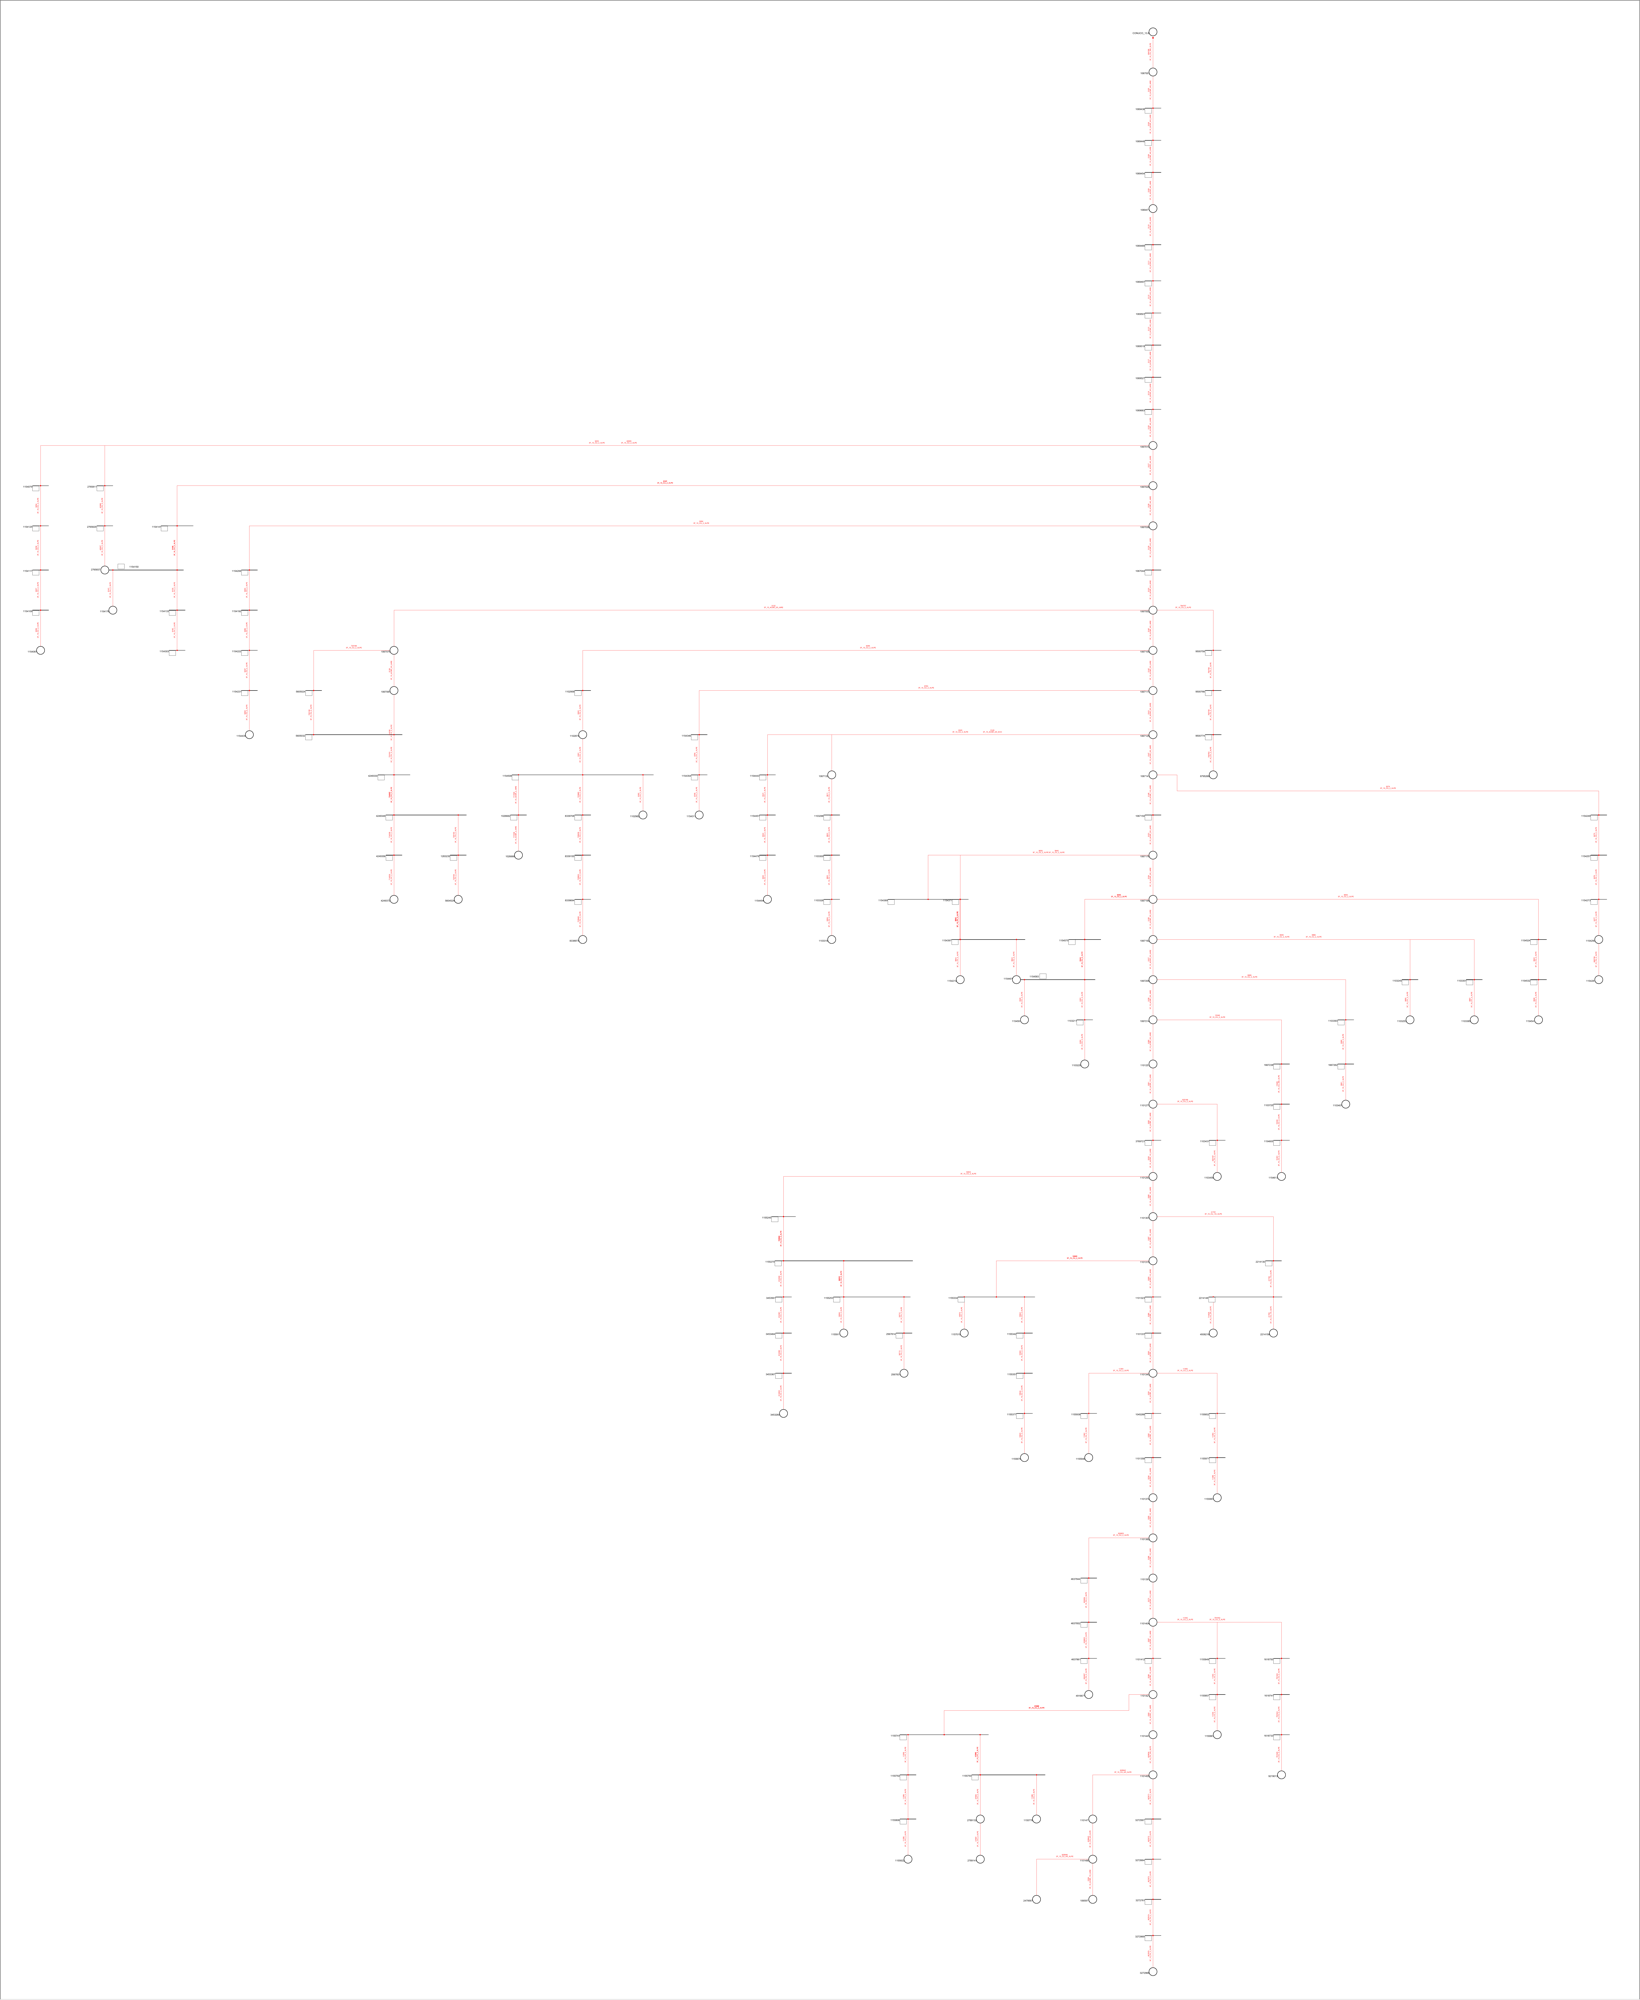
\includegraphics[width=\textwidth,height=0.72\textheight,keepaspectratio]{figuras/cto_10502-1.png}
    \caption{Diagrama unifilar del circuito 10-502 (fuente: ESSA)}
    \label{fig:unifilar}
\end{figure}
\clearpage

\section{Esquema de Componentes del Proyecto}

\begin{center}
    \begin{tabular}{c}
    \toprule
    \textbf{COMPONENTES DEL SISTEMA} \\
    \midrule
    \\
    Paneles Fotovoltaicos \\
    (240 $\times$ 590 W = 141,6 kWp) \\
    \textbar \\
    Inversores SOLIS \\
    (2 $\times$ 60 kW = 120 kW AC) \\
    \textbar \\
    Protección de Inversor \\
    (3 $\times$ 140--200 A) \\
    \textbar \\
    Protección de Acometida \\
    (3 $\times$ 350--500 A) \\
    \textbar \\
    Transformador de Conexión \\
    (150 kVA, 13,2 kV/220 V, Dyn5) \\
    \textbar \\
    Red de ESSA --- Circuito 10-502 \\
    (Nodo 3272966, 13,8 kV) \\
    \\
    \bottomrule
    \end{tabular}
\end{center}

\section{Perfil Horario Completo de Demanda}

\begin{table}[H]
    \centering
    \small
    \caption{Demanda en cabecera del circuito 10-502 (19/03/2024)}
    \begin{tabular}{ccc}
    \toprule
    \textbf{Hora} & \textbf{I [A]} & \textbf{S [MVA]} \\
    \midrule
    00:00 & 34,99 & 0,836 \\
    01:00 & 33,26 & 0,795 \\
    02:00 & 31,86 & 0,762 \\
    03:00 & 28,46 & 0,680 \\
    04:00 & 26,35 & 0,630 \\
    05:00 & 26,78 & 0,640 \\
    06:00 & 29,72 & 0,710 \\
    07:00 & 35,62 & 0,851 \\
    08:00 & 50,59 & 1,209 \\
    09:00 & 61,05 & 1,459 \\
    10:00 & 66,21 & 1,583 \\
    11:00 & 69,70 & 1,666 \\
    12:00 & 70,41 & 1,683 \\
    13:00 & 67,38 & 1,611 \\
    14:00 & 64,58 & 1,544 \\
    15:00 & 68,55 & 1,638 \\
    16:00 & 68,78 & 1,644 \\
    17:00 & 67,10 & 1,604 \\
    18:00 & 62,31 & 1,489 \\
    19:00 & 55,36 & 1,323 \\
    20:00 & 49,48 & 1,183 \\
    21:00 & 44,82 & 1,071 \\
    22:00 & 40,30 & 0,963 \\
    23:00 & 37,40 & 0,894 \\
    \bottomrule
    \end{tabular}
\end{table}

\section{Especificaciones Técnicas Resumen}

\begin{table}[H]
    \centering
    \caption{Especificaciones técnicas generales del proyecto}
    \begin{tabular}{ll}
    \toprule
    \textbf{Parámetro} & \textbf{Valor} \\
    \midrule
    Ubicación & Bucaramanga, Santander \\
    Latitud / Longitud & 7,12621563° / $-$73,11227598° \\
    Capacidad instalada DC / AC & 141,6 kWp / 120 kW \\
    Tecnología & Paneles monocristalinos JINKO \\
    Número de paneles / potencia & 240 / 590 W \\
    Eficiencia de paneles & 22,84\% \\
    Inversores & 2 $\times$ SOLIS 60K-LV-5G \\
    Factor de potencia & 0,99 \\
    Tensión de salida & 220 VAC, 60 Hz \\
    Relación DC/AC & 1,18 \\
    Transformador & 150 kVA, 13,2/0,22 kV, Dyn5 \\
    Circuito / POC & 10-502 / Nodo 3272966 \\
    Nivel de tensión conexión & 13,8 kV \\
    Año de entrada en operación & 2025 \\
    \bottomrule
    \end{tabular}
\end{table}

\section{Matriz de Evaluación de Impacto}

\begin{table}[H]
    \centering
    \caption{Evaluación de impacto en parámetros del sistema}
    \begin{tabular}{lcccc}
    \toprule
    \textbf{Parámetro} & \textbf{Límite} & \textbf{Máximo} & \textbf{Cumple} & \textbf{Impacto} \\
    \midrule
    Tensión (p.u.) & 0,90--1,10 & 0,9953 & $\checkmark$ & Mínimo \\
    Cargabilidad líneas (\%) & $\leq$ 100 & 4,57 & $\checkmark$ & Mínimo \\
    Cargabilidad trafo (\%) & $\leq$ 100 & 55,83 & $\checkmark$ & Bajo \\
    Variación CC & $<$ 1\% & $\approx$0\% & $\checkmark$ & Nulo \\
    Factor de potencia & $\geq$ 0,90 & 0,99 & $\checkmark$ & Positivo \\
    Pérdidas técnicas (kW) & Reducción & $-$0,34 & $\checkmark$ & Positivo \\
    \bottomrule
    \end{tabular}
\end{table}

\section{Cronograma de Validación Recomendado}

\begin{table}[H]
    \centering
    \caption{Actividades de validación post-conexión}
    \begin{tabular}{llcl}
    \toprule
    \textbf{Fase} & \textbf{Actividad} & \textbf{Plazo} & \textbf{Responsable} \\
    \midrule
    Pre-operación & Inspección de instalaciones & 2 semanas & COPOWER + ESSA \\
    Pre-operación & Pruebas de protecciones & 2 semanas & COPOWER + ESSA \\
    Operación & Mediciones de calidad & 1 mes & COPOWER + ESSA \\
    Operación & Validación de tensiones & 3 meses & ESSA \\
    Operación & Reporte de desempeño & Trimestral & COPOWER \\
    \bottomrule
    \end{tabular}
\end{table}

\section{Documentos de Referencia}

\begin{itemize}
    \item Resolución CREG 030 de 2018 --- Conexión de generadores
    \item Resolución CREG 025 de 1995 --- Código de Redes
    \item Resolución CREG 174 de 2021 --- Autogeneración a pequeña escala
    \item Acuerdo 1322 del CNO --- Protecciones de generadores
    \item Norma IEC 60909 --- Cálculo de cortocircuito
    \item Norma IEEE 242 --- Protecciones de sistemas
    \item Datos Circuito 10 502 - 2026.xlsx (ESSA)
    \item Diagrama CTO 10 502.pdf (ESSA)
    \item Ficha técnica inversor SOLIS 60K-LV-5G
    \item Ficha técnica paneles JINKO Monocristalinos
\end{itemize}

\section{Contacto}

\begin{center}
    \textbf{COPOWER LTDA} \\
    Especialistas en Energías Renovables \\
    Bucaramanga, Santander --- Colombia \\
    Julio de 2026
\end{center}
